\subsection{From the GGM84 generic PRF}
The study of \textit{puncturable} or \textit{constrained} PRFs was initiated independently by \cite{AC:BonWat13, CCS:KPTZ13, PKC:BoyGolIva14}.
Here we recall a simple construction in \cite[Section 4.1]{CCS:KPTZ13} building on the \cite{FOCS:GolGolMic84} PRF from a PRG $G$ with factor $2$ expansion.
See Figure~\ref{fig:GGM84:tree_based_prf} for an intuitive representation of such scheme.
The main idea to puncture such PRF at a given point is to replace the PRF key, namely the PRF seed stored in the root of binary tree, with the seeds stored in the co-path associated to the punctured point.


\begin{figure}[htb]
	\centering
	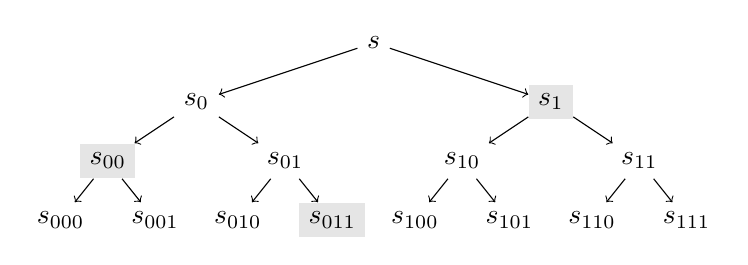
\begin{tikzpicture}[xscale=1.5, yscale=-.75]
	\tikzstyle{hl}=[fill=black!10!]
		\node (s) at (0,0) {$s$};
		
		\node (s0) at (-1.5, 1) {$s_0$};
		\node[hl] (s1) at (1.5, 1) {$s_1$};
		
		\node[hl] (s00) at (-2.25, 2) {$s_{00}$};
		\node (s01) at (-0.75, 2) {$s_{01}$};
		\node (s10) at (0.75, 2) {$s_{10}$};
		\node (s11) at (2.25, 2) {$s_{11}$};
		
		\node (s000) at (-2.25-.4, 3) {$s_{000}$};
		\node (s001) at (-2.25+.4, 3) {$s_{001}$};
		\node (s010) at (-0.75-.4, 3) {$s_{010}$};
		\node[hl] (s011) at (-0.75+.4, 3) {$s_{011}$};
		\node (s100) at (0.75-.4, 3) {$s_{100}$};
		\node (s101) at (0.75+.4, 3) {$s_{101}$};
		\node (s110) at (2.25-.4, 3) {$s_{110}$};
		\node (s111) at (2.25+.4, 3) {$s_{111}$};
		
		%========================================================================
		% Arrows
		\draw[->] (s) to (s0);
		\draw[->] (s) to (s1);
		
		\draw[->] (s0) to (s00);
		\draw[->] (s0) to (s01);
		\draw[->] (s1) to (s10);
		\draw[->] (s1) to (s11);
		
		\draw[->] (s00) to (s000);
		\draw[->] (s00) to (s001);
		\draw[->] (s01) to (s010);
		\draw[->] (s01) to (s011);
		\draw[->] (s10) to (s100);
		\draw[->] (s10) to (s101);
		\draw[->] (s11) to (s110);
		\draw[->] (s11) to (s111);
	\end{tikzpicture}
	\caption{\cite{CCS:KPTZ13} punctured PRF. Highlighted nodes constitute the key obtained puncturing in $x = (0,1,0)$.}
	\label{fig:KPTZ13:punctured_ggm}
\end{figure}

For ease of presentation we deviate from \cite{CCS:KPTZ13} and only show how to restrict the PRF on \textit{fixed prefix} strings, i.e. given $u \in \{0,1\}^\ell$ and a punctured key for $u$, we can only evaluate it on those $x = (u, v)$ for $v \in \{0,1\}$.
The final construction to puncture on a single point $x^\ast$ follows taking the union of keys for all prefixes $u$ of $x^\ast$ with the last bit of $u$ switched\footnote{In general given punctured keys $(k_1, \ldots, k_n)$ for $S_1, \ldots, S_n$ their union may not be a secure key punctured on $S_1 \cap \ldots \cap S_n$, but in this specific case it is.}.
A full description is provided in Figure~\ref{prot:KPTZ13:prefix_punctured_prf}.
For simplicity of notation, given a string $x = (b_1, \ldots, b_\ell)$ we will denote $G_x = G_{b_\ell} \circ \ldots \circ G_{b_1}$, with $G_0$ and $G_1$ being respectively the first and last $\secp$ bits of $G$'s output.

\begin{figure}[htb]
\centering
\begin{pcarray}{lll}
	\algorithm{
		$\cd{Gen}(1^\secp):$
		}
		{
			Sample a seed $s$
				\\
			\textbf{Return} $(s, \varnothing)$
		}
		&
	\algorithm{
		$\cd{Puncture}((s, \varnothing); u):$
		}
		{
			\textbf{Return} $G_u(s)$
		}
		&
	\algorithm{
		$\cd{Eval}((k, u), x)$
		}
		{
			Parse $x = (u', v)$
				\\
			\textbf{If} $u \neq u'$: \textbf{Return} $\perp$
				\\
			\textbf{Else}: \textbf{Return} $G_{v}(k)$
		}
\end{pcarray}
\caption{Punctured PRF from a PRG $G: \{0,1\}^\secp \to \{0,1\}^{2\secp}$. $G_0$ and $G_1$ on input $s$ returns respectively the first and last $\secp$ bits of $G(s)$. $\varnothing$ is used to denote the empty string.}
\label{prot:KPTZ13:prefix_punctured_prf}
\end{figure}

\begin{theorem}
	\label{theo:KPTZ13:prefix_punctured_prf}
	If $G : \{0,1\}^\secp \to \{0,1\}^{2\secp}$ is a secure PRG, then $(\cd{Gen}, \allowbreak \cd{Puncture}, \allowbreak \cd{Eval})$ is a puncturable PRF for the sets $\{S_u : u \in \cup_{\ell = 1}^n \{0,1\}^\ell\}$ where $S_u = \{x \: : \: \nexists v : x = (u, v)\}$.
\end{theorem}
\begin{proof}
	Correctness easily follows as given a key $s$ and its puncturing $k$ in $S_u$, then for all $x \notin S_u$, i.e. for all strings with prefix $u$, the evaluation with $k$ yields, calling $x = (u, v)$.
	\begin{align*}
		G_{v}(k)
			\; = \;
		G_v \circ G_u (s)
			\; = \;
		G_{(u,v)}(s)
			\; = \;
		G_x(s).
	\end{align*}
	To show pseudorandomness on punctured points, let $(k,u) = \cd{Puncture}(s, u)$ and $x \in S_u$. As $u$ is not a prefix of $x$, let $w$ be longest common prefix of $u$ and $x$.
	Without loss generality we assume the next bit after $w$ of $u$ to be $0$ while for $x$ to be $1$.
	Then we argue using the PRG security that the two distributions
	\[
		(G_{(w,0)}(s), G_{(w,1)}(s))
			, \quad
		(r_0, r_1)
	\]
	are computationally indistinguishable for random $r_0, r_1$. This follows as the first distribution is $G \circ G_w(s)$ that is a composition of PRGs.
	We thus conclude that the following distributions are computationally indistinguishable, where $u = (w, 0, \bar{u})$ and $x = (w, 1, \bar{u})$.
	\[
		\left( G_u(s),  G_x(s) \right)
			\; \equiv_c \;
		\left( G_{\bar{u}}(r_0), G_{\bar{x}}(r_1) \right)
			\; \equiv_c \;
		\left( G_{\bar{u}}(r_0), r^\ast \right)
	\]
	for uniformly sampled and independent $s, r_0, r_1, r^\ast$.
\end{proof}